\documentclass[conference]{IEEEtran}

\usepackage[utf8]{inputenc}
\usepackage[T1]{fontenc} % Use 8-bit encoding that has 256 glyphs
\usepackage[english]{babel} % English language/hyphenation
\usepackage[caption=false,font=footnotesize]{subfig}

\ifCLASSINFOpdf
  \usepackage[pdftex]{graphicx}
  % declare the path(s) where your graphic files are
  \graphicspath{{../pdf/}{../jpeg/}{../static/}}
  % and their extensions so you won't have to specify these with
  % every instance of \includegraphics
  \DeclareGraphicsExtensions{.pdf,.jpeg,.png}
\else
\fi

\usepackage{array}

\usepackage{fixltx2e}

\usepackage{url}

\usepackage{amsmath}

\hyphenation{op-tical net-works semi-conduc-tor}

\usepackage[backend=bibtex]{biblatex}
\bibliography{IEEEabrv,bibfiles/bibtexlibs}

\usepackage{todonotes}
\usepackage{bytefield}

\newcommand{\cm}[1]{
  \todo[inline, color=cyan]{Citation missing: #1}
}

\usepackage{tikz}
\usetikzlibrary{arrows}
\tikzset{vertex/.style = {shape=circle,draw,minimum size=2em}}
\tikzset{edge/.style = {->, > = latex'}}
\tikzset{node distance = 5em}


\begin{document}

% paper title
% Titles are generally capitalized except for words such as a, an, and, as,
% at, but, by, for, in, nor, of, on, or, the, to and up, which are usually
% not capitalized unless they are the first or last word of the title.
% Linebreaks \\ can be used within to get better formatting as desired.
% Do not put math or special symbols in the title.
\title{Reservoir computing med greier?}

\author{
    \IEEEauthorblockN{Aleksander Vognild Burkow}
    \IEEEauthorblockA{
        Department of Computer and Information Science\\
        Norwegian University of Science and Technology\\
        Sem Sælandsvei 7-9, 7491 Trondheim, Norway\\
        \texttt{aleksanderburkow@gmail.com}
    }
}

\maketitle

\listoftodos

\begin{abstract}

Reservoir Computing, a relatively new approach to machine learning,
utilizes untrained Recurrent Neural Nets as a reservoir of dynamics to preprocess some temporal task,
making it separable with a linear readout layer
Originating from the study of Liquid State Machines and Echo State Networks,
potentially any sparsely connected network containing feedforward and feedback loops can be a reservoir.
Random Boolean Networks (RBN) is such a sparsely connected network that may be suitable for Reservoir Computing.

In this paper we investigate the dynamics, performance, and viability of RBNs used for Reservoir Computing (RRC).
A system to investigate these properties is implemented,
and its correctness is validated by comparing its results with those of comparable studies.
The chosen reproduced experiments result in the following findings:
The more chaotic the phase of an RBN is, the higher its required input connectivity.
The value of $K$ which provides optimal computational power is found to lie closer to $K=3$ when using homogenous networks,
as opposed to the heterogenous optimal $\langle K \rangle = 2$.
A relationship between Computational Capability and actual reservoir performance seems to exist.

Finally, we find a one-to-many mapping between the readout layer in an already-trained RRC system and different RBN reservoirs,
with there being a seemingly large set of interchangeable reservoirs for each readout layer.
This makes the potential use of a smaller generative genome for evolving RRC systems interesting.
Even though it hits fewer points in the RBN fitness landscape than the fixed genome used in this paper,
a large amount of these points are still usable for each instance of a working readout layer.

\end{abstract}


\section{Introduction}

Reservoir computing (RC) is a form of machine learning that sprung out from the study of recurrent neural networks (RNNs).
In short, it utilizes the dynamics of some complex system dubbed a 'reservoir' to preprocess a timeseries problem,
transforming it from a temporal to a spacial one in the reservoir, making it then separable with a usually simple readout layer.

In this paper we investigate the dynamics of Reservoir Computing systems where the reservoir is a Random Boolean Network (RBN) \cite{gershenson2004introduction},
an approach found fruitful in \cite{rbn-reservoir}.

First we reproduce chosen experiments from \cite{rbn-reservoir}, creating a working RBN-reservoir computing system (RRC).

Next we investigate whether the readout layer of a working RRC system can be re-used with other RBN-reservoirs than the one it was trained on,
and still stay accurate on the original classification task.
These functionally equivalent reservoirs will be found through the use of an evolutionary algorithm.

Last we look at the dynamics and characteristics of these groups of RBN-Reservoirs, attempting to find any similarities that might be exploitable.

\subsection{A brief introduction to reservoir computing}

Recurrent neural networks, as opposed to feed-forward neural networks,
are notoriously time consuming and difficult to train.
This due to feedback from the recurrent connections during the training process,
allowing small topology changes to drastically change ones position in the fitness landscape.

It was therefore proposed both in \cite{jaeger2002adaptive} (as echo state networks, or ESN)
and \cite{natschlager2002liquid} (as liquid state machines, or LSM) to separate the RNN into two parts,
the untrained reccurrent reservoir, and the trained readout layer.
Both of these methods have been unified into the field of Reservoir Computing,
now focusing on the separate training and evolution of the recurrent and readout part \cite{lukovsevivcius2012reservoir}.

Useful RC resources include Organic \cite{organic}, an online RC hub,
providing documentation, references, and a RC toolbox implemented in python.
It has been quite useful for this project.
Exiting applications of reservoir computing include speech and handwriting recognition,
as well as controlling robotics, as detailed in \cite{lukovsevivcius2012reservoir}.

\subsection{Alternatives to classical reservoirs}

An interesting question arises:
Are there other types of complex systems that can be used as reservoirs?
What properties must these reservoirs have to be able to solve problems?

Complex networks similar to the sparsely connected RNNs found in classical RC devices include Cellular Automata and Random Boolean Networks.
Both are considerably less complex than RNNs, requiring only simple lookup tables for state transitions as opposed to multiplication for RNNs.
A short treatise on Cellular Computing \& friends is available here \cite{sipper1999emergence}.
Cellular computing provides a potentially powerful alternative to classical computers,
leveraging extreme parallelism, simple components and local state.

The ever-so-cited 'Water bucket' paper investigated the use of an actual bucket of water as a reservoir \cite{fernando2003pattern},
successfully recognizing patterns and achieving decent performance at that.
The RBN-reservoir \cite{rbn-reservoir} approach mentioned earlier, has also been found to be viable.

\subsection{Dynamics and complexity of reservoirs}

In general, one wishes to use a reservoir with a complexity matching that of the problem.
Utilizing a modern processor to predict a very simple timeseries would be a classic case of shooting sparrows with cannons \cite{wiki:sparrow},
while achieving the same using a RBN or CA might be more impressive.

\todo[inline]{Gotta finish introduction from hereon and down}

So we have all this litterature on complex systems (CITATIONS HERE) that show that optimal computing power is most often found on the 'edge of chaos', or the critical state, on the edge between periodic and chaotic dynamics.
In addition we have a measure for computational power in RRN's developed in \cite{rbn-reservoir} that awards good scores to networks that are able to both separate two at-some-point similar input sequences, as well as two sequences that used to differ in the past.
They show that this measure too, is maximized at critical connectivity (K=2) for RBNs.

% HERE I WRITTEN TTTO

These reservoirs have dynamics which can be analysed.
So if we find other networks with different topologies but similar dynamics,
we should be able to use this new network as the 'reservoir' with a simple readout layer.

If this area of research remains fruitful,
it can be used to develop metrics for what other 'reservoirs' or even physical materials might be useful as a computational base.
This can be useful for evolution in materio, for selecting substrates \cite{evolutionInMaterio}

\subsection{What i actually done in this paper?}

A rbn-simulator was developed in the Python programming language,
using the following things for glue, regression, inspiration, and duct-tape.

\begin{itemize}
  \item MDP + Oger for putting nodes in a flow, and regressing
  \item Numpy + Scipy for numerical calculations, array backing
  \item RBN Matlab toolbox for inspiration
  \item Homegrown RBN-simulator, Evolutionary alogrithm borrowed from friend
\end{itemize}


\section{Background}

\subsection{A brief introduction to boolean networks}

Random Boolean Networks, also known as Kaffman networks, were originally developed as a model of genetic regulatory networks \cite{kauffman1969metabolic}.
The model makes no assumptions about the actual functioning of the nodes in the network,
making them useful to model a wide range of phenomena.
The simplification of a system to a boolean model doesn't pose a problem,
as any multi-valued network can be transformed to a corresponding binary one.

A RBN is usually described by its number of nodes $N$ and the in-degree $K$ of the nodes,
that is, how many nodes each node depends on (also known as its ancestors).
RBNs can have both homogenous and heterogenous in-degrees.
In heterogenous networks, one usually describes the average connectivity $<K>$ instead.

Each node can have a state of zero or one.
The next state of the node is solely determined by the current combination of states of its ancestors.
Each combination leads to a new state of zero or one,
with the probability given by a binomial distribution usually having $<p>=0.5$.
Figure \ref{figure:sample-homogenous-rbn} visualizes a homogenous RBN with N=3 K=2, and P=0.5.

\begin{figure}
  \centering
  \subfloat[RBN topology]{
    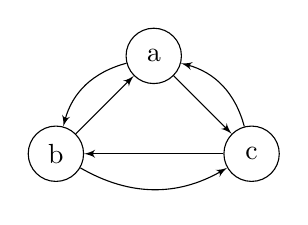
\begin{tikzpicture}[node distance = 5em]
      \node[vertex] (a) {a};
      \node[vertex] (b) [below left of=a] {b};
      \node[vertex] (c) [below right of=a] {c};

      \draw[edge] (a) to[bend right] (b);
      \draw[edge] (a) to (c);

      \draw[edge] (b) to (a);
      \draw[edge] (b) to[bend right] (c);

      \draw[edge] (c) to[bend right] (a);
      \draw[edge] (c) to (b);
    \end{tikzpicture}
  }
  \subfloat[Transition table for node a]{
    \begin{tabular}[b]{ c c | c}
      \multicolumn{2}{c}{Ancestor states} & New state \\
      \hline
      0 & 0 & 0 \\
      0 & 1 & 1 \\
      1 & 0 & 0 \\
      1 & 1 & 1 \\
    \end{tabular}
  }
  \caption{An example homogenous RBN with N=3, K=2.}
  \label{figure:sample-homogenous-rbn}
\end{figure}

In the classical RBN model (CRBN), all nodes update at the same time,
therefore the states of the network at $t+1$ only depends on the states at $t$.
This is a simplification that isn't quite accurate for all systems,
notably gene regulation networks where the system doesn't operate in lockstep.
There are therefore a number of updating schemes on the spectrum of determinism and randomness.

The dynamics of an RBN can be categorized as being in either the ordered, critical, or chaotic phase.
These phases can be identified by how large a part of the network state is able to change over time,
whether similar states tend to converge or diverge over time,
and the networks resistance to perturbations (outside changes to the network).

As these phases are easy to identify visually,
we will plot the states of the RBN in a square lattice,
with the network states plotted horizontally, and time flowing downwards.
A node is drawn as white if its state is one, black otherwise.
The phases are visualized in figure \ref{figure:rbn-phases}.

\begin{figure}
  \subfloat[Ordered phase, K=1]{
    
\includegraphics[width=0.3\columnwidth]{background/ordered-phase.pdf}
    \label{figure:rbn-ordered}
  }
  \subfloat[Critical phase, K=2]{
    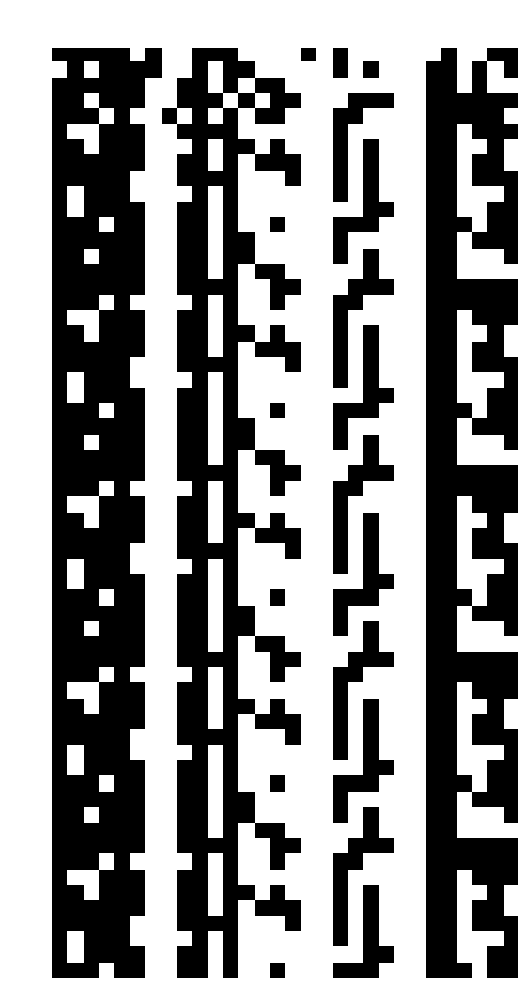
\includegraphics[width=0.3\columnwidth]{background/critical-phase.pdf}
    \label{figure:rbn-critical}
  }
  \subfloat[Chaotic phase, K=3]{
    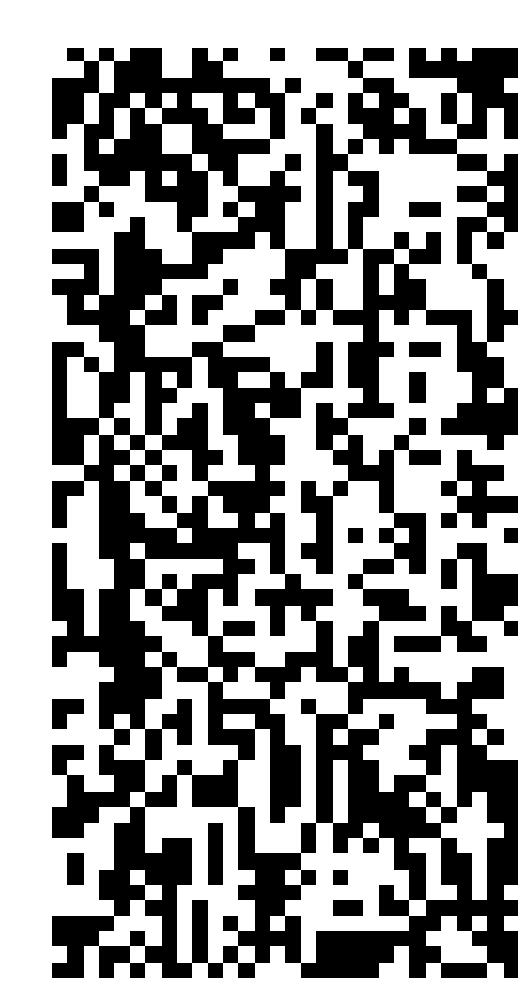
\includegraphics[width=0.3\columnwidth]{background/chaotic-phase.pdf}
    \label{figure:rbn-chaotic}
  }

  \caption{
    Trajectories through state-space for RBNs with $N=30, K=[1,2,3]$, visualizing the different phases.
    Images created with the developed RBN-simulator.
  }
  \label{figure:rbn-phases}
\end{figure}

In general, RBNs in the critical phase are the most interesting.
These are seemingly able to support both information transmission, storage and modification,
capacities required for computation \cite{langton3computation}.
Critical systems are found on the edge of chaos, on the phase transition between ordered and chaotic networks.
For classical RBNs with $<p>=0.5$, critical networks are usually found at $<K>=2$ \cite{gershenson2004introduction},
although one could still create networks with similar dynamics for different $K$.

A thorough introduction to the field of RBNs is available in \cite{gershenson2004introduction}.

\subsection{RBN-Reservoir systems}
\label{subsection:rbn-reservoir-systems}

How does one adapt a RBN for use as a reservoir in a RBN-RC device?
RBNs aren't usually designed to take external input.
We do however, have the concept of perturbation,
the external flipping of bits in the networks state,
transition tables or edges.
This can be utilized to create RBNs that take input,
by continiously perturbing the RBN nodes by the bits of the input sequence.

Questions that follow are how many bits should the network consume at a time,
how many of the network nodes should be perturbed by the input at each timestep,
and what dynamics must such a reservoir have to allow for the computation of interesting problems?

\subsubsection{A working system}

In \cite{rbn-reservoir} the authors create and analyze functioning RBN-RC systems.
These RBN-RC systems have heterogenous connectivity,
consume one bit of input at each timestep ($I=1$),
perturbing $L$ of the $N$ nodes in the process.
The readout layer can be any node performing some kind of regression of the reservoir state against expected outout for the current task, e.g. linear regression.
Such a setup is shown in figure \ref{figure:rbn-reservoir}.

\begin{figure}
  \centering
  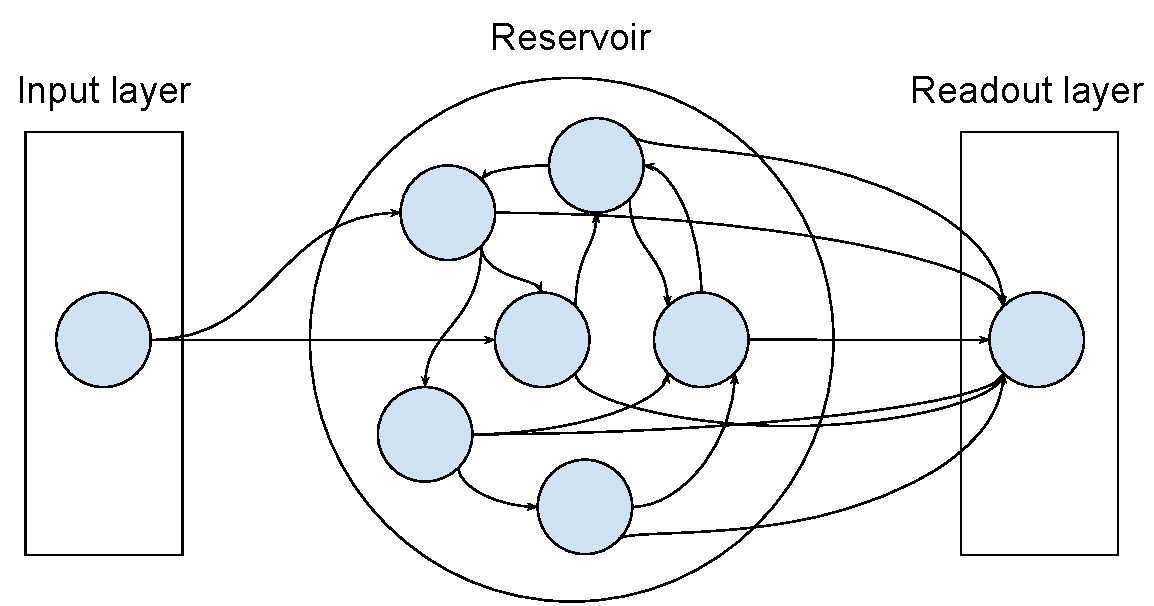
\includegraphics[width=\columnwidth]{background/RBN-Reservoir.pdf}
  \caption{
    RBN-Reservoir system with $I=1, L=2, K=2, N=5$.
    The reservoir transforms the problem from a temporal one to a multidimentional spatial one.
    The readout layer the performs some kind of learning on the reservoir states against the expected output for the current task.}
  \label{figure:rbn-reservoir}
\end{figure}

\subsubsection{Tasks}

To measure the real-life performance and accuracy of the RBN-reservoir systems, two tasks were introduced: Temporal Density and Temporal Parity \cite{rbn-reservoir}.
Both require the reservoir to be able to retain information for a sliding window of size $ n $,
offset by some value $ t $, back through the input stream.
The temporal Parity task requires us to determine if there were an odd number of ones in the sliding window,
the temporal density task to determine whether there were a majority of ones.
The former is visualized in figure \ref{figure:temporal-parity},
and will be used to benchmark the reservoirs created later in this paper.

\begin{figure}
  \subfloat[Input]{
    
\includegraphics[width=\columnwidth]{background/temporal_parity-10-200-3-input.pdf}
  }

  \subfloat[Correct output]{
    
\includegraphics[width=\columnwidth]{background/temporal_parity-10-200-3-output.pdf}
  }

  \caption{
    The first 30 elements of a Temporal Parity task with $[n=3, t=0]$.
    A one is visualized as white, while a zero is black.
    We see that correct output at time $i$ is equal to there being an odd number of $1$s in inputs $[i, i-1, i-2]$
  }
  \label{figure:temporal-parity}
\end{figure}

\subsubsection{Computational capability}
\label{section:computational-capability}
For an RBN-reservoir to perform well in computational tasks,
it must be able to both forget past perturbations and separate input streams that have started converging.

These two properties are coined \textit{fading memory} and \textit{separation property} \cite{rbn-reservoir},
and can be measured as follows.
Create two equal input streams \#1 and \#2 of length $T$.
If measuring \textit{fading memory}, flip the first bit in stream \#2.
If measuring \textit{separation property}, flip all bits up to bit $T-t$ in stream \#2
($t$ being the required depth of separation).
For both input streams, reset reservoir state, perturb the reservoir with the input stream,
and store the final state.
The score of the measure is then defined as the normalized hamming distance between the resulting states.
The computational capability $\Delta$ of an RBN-reservoir is then defined as
\begin{equation}
  \Delta_{Tt} = separation\_property_{Tt} - fading\_memory_{T}
\label{formula:accuracy}
\end{equation}

Analyzing different RBN-reservoirs with this metric \cite{rbn-reservoir},
a high $\Delta$ is found to correlate with critical connectivity ($<K>=2$).
For all RBN-reservoirs, $\Delta$ drops when increasing the required separation $t$,
and is maximized when one doesn't have to remember anything at all ($t=0$).

\subsubsection{Optimal perturbance}
It is found that the optimal amount of reservoir perturbance,
adjustable by the number of connections between the input layer and the reservoir,
depends on both the task size, how many steps in time are required to be remembered,
and the dynamics of the reservoir.
\textit{Chaotic reservoirs} require few input connections to be able to properly spread information,
but perform poorly on larger tasks due to past perturbations still floating around the reservoir.
\textit{Ordered reservoirs} quickly forget past perturbations, allowing some success for larger tasks,
but their inability to remember past perturbations renders them useless for many tasks.
\textit{Critical reservoirs} require connectivity somewhere in the middle.
Able to forget as well as remember, they perform accurately independent of task size.


\section{Method}

To verify the viability of RBNs in RC systems, a functioning RRC system has to be created.
Being able to reproduce results from \cite{rbn-reservoir} will lend credibility to the approach presented in this paper.
The Computational Capability measure presented therein will be used to analyze our RRC systems.

Second, we wish to investigate the potential many-to-many relationship betwen readout layers and reservoirs,
evolving these functionally equivalent reservoirs through artificial evolution.
These sets of interchangeable reservoirs may share similar attributes and Computational Capability,
and will be analyzed.
If such a mapping exists it may tell us something about how large a part of the RBN fitness landscape is usable as a reservoir, and how difficult it is to reach these points.
A smaller generative genome could then be used instead of the fixed one presented in this paper,
potentially guided towards the attributes we find useful.

The following systems have been implemented to investigate the stated questions:
\begin{itemize}
  \item An RBN simulator
  \item Procedures for analyzing and visualizing RBNs
  \item Procedures for creating classification tasks

  \item An RBN Reservoir Computing system using:
  \begin{itemize}
    \item The aforementioned RBN simulator as a reservoir
    \item The ridge regression node from the Oger RC toolkit \cite{verstraeten2012oger} as readout layer
    \item The Python Modular Toolkit for Data Processing \cite{zito2008modular} for glue and training of the RRC system.
  \end{itemize}
  \item A system for evolving RBNs given certain constraints, using a genetic algorithm based on the one used in \cite{farstad2015evolving}.
\end{itemize}

The codebase is available on GitHub \cite{forprosjekt-code-github} under a soon-to-be permissive licence.

\subsection{Measuring Computational Capability}

We will be using the computational complexity measure introduced in \ref{section:computational-capability} to analyze the created RBNs.
This measure is parameterized over both input stream length $T$ and the required depth of separation $t$.
To make this an useful measure when comparing against reservoir accuracy on a specific task,
we will chose values of $T$ similar to the length and $t$ equal to the required memory of that task.

\subsection{The creation and training of a functioning RRC system}

The final RRC system is shown as a block diagram in Figure \ref{figure:rrc-block},
and the actual network topology is equivalent to the one in Figure \ref{figure:rbn-reservoir}.

\begin{figure}
  \centering
  \begin{tikzpicture}
    \node (dataset) {Dataset};
    \node[box, below=of dataset] (input) {Input layer};
    \node[box, right=of input] (reservoir) {RBN Reservoir};
    \node[box, right=of reservoir] (readout) {Readout layer};
    \node[above=of readout] (classification) {Classification};

    \node[draw,dotted,fit=(input) (reservoir) (readout), label={RRC}] {};

    \draw[edge] (dataset) to (input);
    \draw[edge] (input) to (reservoir);
    \draw[edge] (reservoir) to (readout);
    \draw[edge] (readout) to (classification);
  \end{tikzpicture}
  \caption{Block diagram of the RRC processing a dataset.}
  \label{figure:rrc-block}
\end{figure}

\subsubsection{testing}

To verify that RBN simulation is working,
a RBN is created randomly, initial state set to all zeros, and ran.
The results are visualized in Figure \ref{figure:rbn-noperturb}.
We see that the RBN exhibits stable dynamics, and enters into an attractor around $t=15$.
In Figure \ref{figure:rbn-perturb} we continiously perturb the RBN with the input stream from the Temporal Parity task visualized in Figure \ref{figure:temporal-parity}.
In the perturbed case, the state trajectory is continiously changed, preventing the RBN from settling into an attractor.
Interestingly enough, there seems to be a visual similarity between the two cases.
Such a pattern is sure to dissapear with a RBN in the chaotic phase.

This erratic pattern of state transitions is then fed into the readout layer,
which is then tasked with finding a linear combination of the RBN states that results in the expected output for the given task.

\begin{figure}
  \subfloat[Unperturbed]{
    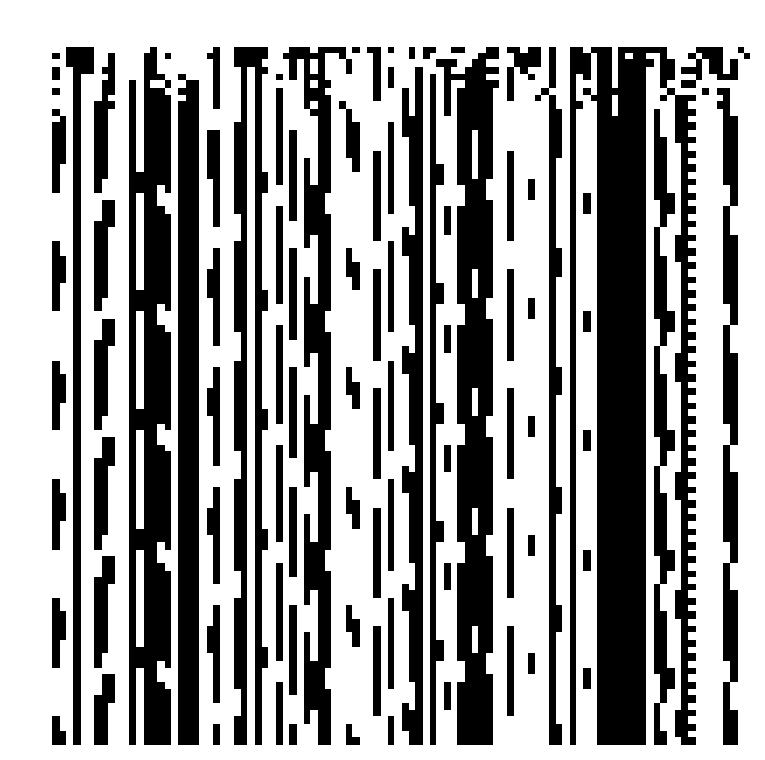
\includegraphics[width=0.5\columnwidth]{method/final-1-noperturb.pdf}
    \label{figure:rbn-noperturb}
  }
  \subfloat[Perturbed]{
    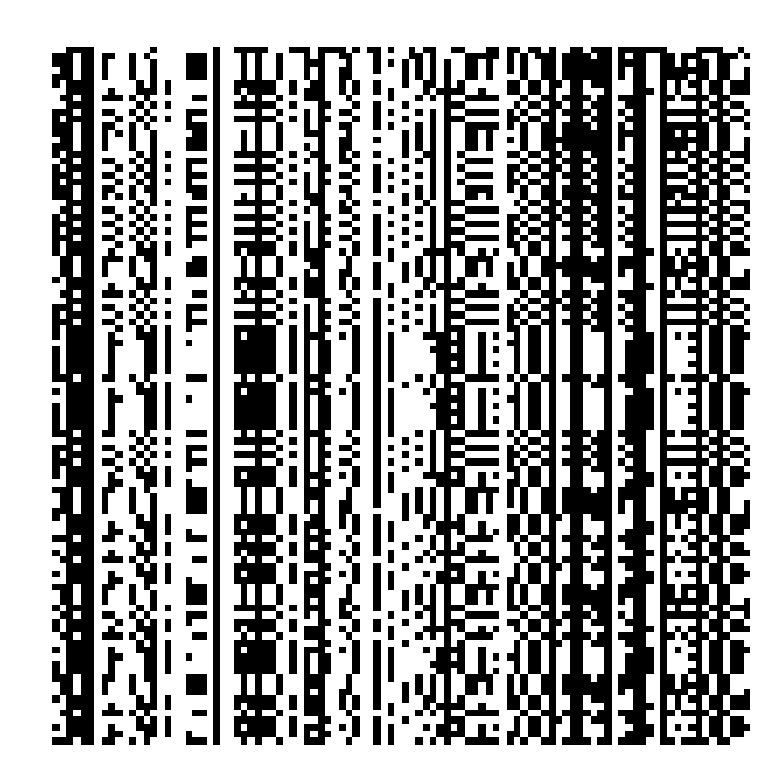
\includegraphics[width=0.5\columnwidth]{method/final-1-perturb.pdf}
    \label{figure:rbn-perturb}
  }
  \caption{
    The same RBN ($N=100, K=2, P=0.5, L=50$) shown both perturbed and unperturbed.
    The boolean states of the RBN are plotted along the X-axis,
    with time flowing downwards.
  }
\end{figure}

\subsubsection{Training}

To train the RRC system we require a number of training datasets,
as well as different testing datasets to test the trained system.
We will use the datasets described in section \ref{subsection:rbn-reservoir-systems}.

We then either create a new RBN (initialize it randomly),
or load a previously created RBN from disk.
For each bit of input in each dataset,
we perturb the input-connected nodes in the RBN.
After each perturbance, the RBN is ran synchronously (CRBN mode) for one timestep.
The resulting RBN states are collected,
and after the entire dataset is processed,
forwarded to the readout layer.

To find a suitable mapping from the set of reservoir states and the correct input classification,
ridge regression \cite{hoerl1970ridge} is used.
This version of least squares regression is more accurate when faced with input colinearities,
as well as always being at least as accurate as ordinary least squares.

This process is repeated for all the datasets,
and the final regression parameters are chosen as a combination of the parameters obtained for each individual dataset.
Finally we measure the normalized accuracy of the trained reservoir on the test dataset,
defined as
\todo[inline]{Use symbols instead of words?}
\begin{equation}
Accuracy = 1 - \dfrac{sum(actual\_output \neq expected\_output)}{len(correct\_output)}
\label{formula:accuracy}
\end{equation}
.
If the RRC system achieves a high accuracy on an interesting task,
it will be stored for further research.

\subsection{The evolving of functionally equivalent RBN reservoirs for existing readout layers}
\label{section:method:evolving-rbns}

To investigate the potential many-to-many mapping between RBN-reservoirs and readout layers,
a Genetic Algorithm (section \ref{section:background:ga}) will be used.
A fixed test dataset and readout layer for fitness evaluation will be used.

\subsubsection{Genotype and phenotype representation}

We let the genotype be a direct encoding of the corresponding RBN graph.
Such an encoding is significantly larger than a generative encoding,
but less complex as well as able to generate all individuals in the fitness landscape.

Each node needs to represent whether it is connected to the input node,
who its neighbors are, and what its transition rule is.
As we only look at homogenous RBNs,
we can use a fixed-length genome with
\begin{equation}
genome\_length = n\_nodes \cdot (connectivity + 2)
\end{equation}
To further simplify GA implementation,
we let all symbols in the genome take a value in the range $[0, max\_required\_in\_genome)$.
The actual symbol values are then computed modulo the largest actual value they could take on
(2 for input connectivity, n\_nodes for neighbors, $2^{2^{n\_nodes}}$ for transition rules).
This redundancy in the genome can be an advantage,
as it allows for new ways to explore the fitness landscape \cm.

The final genome is shown in figure \ref{figure:rbn-genotype}.
Note that this representation sets no limitations on input connectivity or uniqueness of neighbors.

\begin{figure}
  \centering
  \begin{bytefield}[bitwidth=1.5em]{12}
    \bitheader{0-11} \\
    \bitbox{1}{C} \bitbox{1}{N\textsubscript{1}} \bitbox{1}{N\textsubscript{2}} \bitbox{1}{R}
    \bitbox{1}{C} \bitbox{1}{N\textsubscript{1}} \bitbox{1}{N\textsubscript{2}} \bitbox{1}{R}
    \bitbox{1}{C} \bitbox{1}{N\textsubscript{1}} \bitbox{1}{N\textsubscript{2}} \bitbox{1}{R} \\
    \bitbox[t]{4}{$\underbrace{\hspace{6em}}_{\text{\normalsize Node 1}}$}
    \bitbox[t]{4}{$\underbrace{\hspace{6em}}_{\text{\normalsize Node 2}}$}
    \bitbox[t]{4}{$\underbrace{\hspace{6em}}_{\text{\normalsize Node 3}}$} \\
  \end{bytefield}
  \caption{
    The direct-encoded genotype used for evolving RBNs,
    shown here for an RBN with $N=3, K=2$.}
  \label{figure:rbn-genotype}
\end{figure}

\subsubsection{Fitness function}

Each GA run is parameterized with an already-trained and accurate readout layer (separated from its RBN-reservoir),
as well as a single test dataset of the same origins as the dataset used for training the readout layer.
After converting each genotype to its corresponding phenotype,
the resulting RBN is connected to the readout-layer and fed with the fixed test dataset.
The accuracy obtained,
as calculated in formula \ref{formula:accuracy},
is used as the fitness of the phenotype.

\subsubsection{GA hyperparameters}

The hyperparameters for the GA are presented in table \ref{table:ga-hyperparameters}.

\begin{table}
  \centering
  \caption{GA hyperparameters}
  \label{table:ga-hyperparameters}
  \begin{tabular}{ll}
    Children pool size             & 40                                    \\
    Adult pool size                & 40                                    \\
    Fitness satisfaction threshold & 0.98                                  \\
    maximum generations            & 200                                   \\
    Adult selection                & Generational mixing                   \\
    Parent selection               & Tournament selection(K=8)             \\
    Genome crossover               & Per component crossover (p=0.5)       \\
    Genome mutation                & Per genome component mutation (p=0.1) \\
  \end{tabular}
\end{table}

Adult selection is simple generational mixing,
selecting the best 40 specimens from the combined children and adult populations.
Per component crossover will with a probability p either pass through the entire genome from the left parent,
or for each component chose either the left or right parents value with a probability 0.5.
Per genome component mutation will reroll each genome component with probability p.
This value is set relatively high (0.1) due to experiments showing a much faster convergence rate fr this domain than with the initial chosen value of 0.01.


\section{Experiments}

\subsection{Reproduce previous results}

In \cite{rbn-reservoir} the authors find a relationship between computational capability and performance,
that certain values of $L$ give the best reservoir performance,
and that RBNs with connectivity $\langle K \rangle =2$ should outperform other connectivities.
To test these assertions,
we must create and benchmark a number of functioning RBN reservoir systems,
noting their accuracy on the chosen task as well as their computational capability.

We will be using two versions of the \textit{temporal parity} task
(as specified in table \ref{table:task-parameters}) to measure reservoir performance.
The temporal parity task is chosen over temporal density as it is the more difficult task
(shown in \cite{rbn-reservoir}), presumably resulting in more interesting and rich resevoirs.

\begin{table}
  \centering
  \caption{Task parameters}
  \label{table:task-parameters}
  \begin{tabular}{ll}
    Task type         & Temporal Parity \\
    Num. datasets     & 10              \\
    Dataset length    & 200             \\
    $N$ (window size) & 3 and 5         \\
    $t$ (offset)      & 0               \\
  \end{tabular}
\end{table}


As the number of different RBNs is oppressively large,
$(\frac{2^{2^{K}}N!}{(N-K)!})^N$ \cite{gershenson2004introduction},
we therefore create 30 random specimens for each combination of the RBN parameters displayed in table \ref{table:rbn-combinations}.

\begin{table}
  \centering
  \caption{RBN combinations}
  \label{table:rbn-combinations}
  \begin{tabular}{ll}
    N (nodes)              & 100             \\
    K (connectivity)       & 1, 2, 3         \\
    L (input connectivity) & 0, 10, ..., 100 \\
    Temporal parity        & $N=3,5$ \\
  \end{tabular}
\end{table}

\subsection{Evolving reservoirs to re-use existing readout layers}


\section{Results}

\begin{figure*}[!t]
  \centering
  \resizebox{\textwidth}{!}{
    \subfloat{
      \myboxplot{
% L: 0
\addplot[mark=*, mark=*,boxplot]
table[row sep=\\, y index=0] {
data
0.52 \\
0.52 \\
0.48 \\
0.52 \\
0.52 \\
0.48 \\
0.52 \\
0.52 \\
0.52 \\
0.52 \\
0.47 \\
0.52 \\
0.56 \\
0.52 \\
0.47 \\
0.52 \\
0.52 \\
0.52 \\
0.52 \\
0.52 \\
0.47 \\
0.52 \\
0.48 \\
0.47 \\
0.52 \\
0.43 \\
0.52 \\
0.52 \\
0.47 \\
0.52 \\
};
% L: 1
\addplot[mark=*, mark=*,boxplot]
table[row sep=\\, y index=0] {
data
0.55 \\
0.465 \\
0.47 \\
0.36 \\
0.48 \\
0.465 \\
0.47 \\
0.425 \\
0.47 \\
0.455 \\
0.485 \\
0.475 \\
0.48 \\
0.44 \\
0.465 \\
0.645 \\
0.47 \\
0.48 \\
0.36 \\
0.48 \\
0.36 \\
0.48 \\
0.48 \\
0.465 \\
0.52 \\
0.48 \\
0.495 \\
0.48 \\
0.36 \\
0.475 \\
};
% L: 2
\addplot[mark=*, mark=*,boxplot]
table[row sep=\\, y index=0] {
data
0.465 \\
0.465 \\
0.47 \\
0.36 \\
0.36 \\
0.475 \\
0.48 \\
0.49 \\
0.51 \\
0.48 \\
0.475 \\
0.465 \\
0.465 \\
0.47 \\
0.475 \\
0.465 \\
0.475 \\
0.515 \\
0.48 \\
0.475 \\
0.465 \\
0.465 \\
0.475 \\
0.455 \\
0.455 \\
0.48 \\
0.48 \\
0.475 \\
0.47 \\
0.49 \\
};
% L: 3
\addplot[mark=*, mark=*,boxplot]
table[row sep=\\, y index=0] {
data
0.41 \\
0.47 \\
0.405 \\
0.405 \\
0.54 \\
0.475 \\
0.48 \\
0.5 \\
0.5 \\
0.48 \\
0.4 \\
0.45 \\
0.425 \\
0.485 \\
0.465 \\
0.445 \\
0.355 \\
0.465 \\
0.47 \\
0.475 \\
0.595 \\
0.485 \\
0.525 \\
0.61 \\
0.475 \\
0.645 \\
0.36 \\
0.475 \\
0.49 \\
0.465 \\
};
% L: 4
\addplot[mark=*, mark=*,boxplot]
table[row sep=\\, y index=0] {
data
0.465 \\
0.585 \\
0.645 \\
0.405 \\
0.475 \\
0.465 \\
0.485 \\
0.36 \\
0.465 \\
0.48 \\
0.475 \\
0.545 \\
0.465 \\
0.41 \\
0.485 \\
0.475 \\
0.47 \\
0.465 \\
0.595 \\
0.465 \\
0.41 \\
0.47 \\
0.47 \\
0.495 \\
0.485 \\
0.49 \\
0.465 \\
0.475 \\
0.48 \\
0.48 \\
};
% L: 5
\addplot[mark=*, mark=*,boxplot]
table[row sep=\\, y index=0] {
data
0.465 \\
0.465 \\
0.465 \\
0.57 \\
0.36 \\
0.475 \\
0.465 \\
0.475 \\
0.435 \\
0.475 \\
0.53 \\
0.465 \\
0.48 \\
0.355 \\
0.555 \\
0.47 \\
0.475 \\
0.455 \\
0.465 \\
0.475 \\
0.475 \\
0.475 \\
0.475 \\
0.52 \\
0.425 \\
0.585 \\
0.465 \\
0.465 \\
0.405 \\
0.485 \\
};
% L: 6
\addplot[mark=*, mark=*,boxplot]
table[row sep=\\, y index=0] {
data
0.465 \\
0.54 \\
0.54 \\
0.47 \\
0.475 \\
0.435 \\
0.475 \\
0.405 \\
0.355 \\
0.465 \\
0.465 \\
0.465 \\
0.465 \\
0.47 \\
0.41 \\
0.465 \\
0.465 \\
0.465 \\
0.475 \\
0.475 \\
0.465 \\
0.46 \\
0.645 \\
0.465 \\
0.465 \\
0.475 \\
0.475 \\
0.475 \\
0.465 \\
};
% L: 7
\addplot[mark=*, mark=*,boxplot]
table[row sep=\\, y index=0] {
data
0.465 \\
0.465 \\
0.475 \\
0.645 \\
0.475 \\
0.475 \\
0.465 \\
0.465 \\
0.48 \\
0.465 \\
0.475 \\
0.465 \\
0.395 \\
0.465 \\
0.475 \\
0.465 \\
0.645 \\
0.465 \\
0.475 \\
0.47 \\
0.48 \\
0.475 \\
0.47 \\
0.425 \\
0.475 \\
0.465 \\
0.465 \\
0.475 \\
0.47 \\
0.465 \\
};
% L: 8
\addplot[mark=*,boxplot]
table[row sep=\\, y index=0] {
data
0.465 \\
0.465 \\
0.465 \\
0.465 \\
0.465 \\
0.475 \\
0.465 \\
0.465 \\
0.465 \\
0.465 \\
0.475 \\
0.465 \\
0.475 \\
0.465 \\
0.465 \\
0.48 \\
0.465 \\
0.465 \\
0.475 \\
0.465 \\
0.47 \\
0.475 \\
0.465 \\
0.475 \\
0.465 \\
0.465 \\
0.465 \\
0.475 \\
0.465 \\
0.475 \\
};
% L: 9
\addplot[mark=*,boxplot]
table[row sep=\\, y index=0] {
data
0.475 \\
0.465 \\
0.475 \\
0.36 \\
0.465 \\
0.535 \\
0.465 \\
0.465 \\
0.535 \\
0.475 \\
0.465 \\
0.595 \\
0.475 \\
0.465 \\
0.475 \\
0.475 \\
0.465 \\
0.475 \\
0.475 \\
0.475 \\
0.465 \\
0.465 \\
0.475 \\
0.475 \\
0.475 \\
0.475 \\
0.465 \\
0.535 \\
0.475 \\
0.535 \\
};
% L: 10
\addplot[mark=*,boxplot]
table[row sep=\\, y index=0] {
data
0.535 \\
0.535 \\
0.535 \\
0.535 \\
0.535 \\
0.535 \\
0.535 \\
0.535 \\
0.535 \\
0.535 \\
0.535 \\
0.535 \\
0.535 \\
0.535 \\
0.535 \\
0.535 \\
0.535 \\
0.535 \\
0.535 \\
0.535 \\
0.535 \\
0.535 \\
0.535 \\
0.535 \\
0.535 \\
0.535 \\
0.535 \\
0.535 \\
0.535 \\
0.535 \\
};
}{0.1}

    }
    \subfloat{
      \myboxplot{
% L: 0
\addplot[mark=*, boxplot]
table[row sep=\\, y index=0] {
data
0.545 \\
0.59 \\
0.465 \\
0.465 \\
0.515 \\
0.515 \\
0.515 \\
0.465 \\
0.515 \\
0.515 \\
0.515 \\
0.465 \\
0.59 \\
0.515 \\
0.525 \\
0.515 \\
0.465 \\
0.515 \\
0.545 \\
0.465 \\
0.515 \\
0.56 \\
0.515 \\
0.525 \\
0.465 \\
0.525 \\
0.565 \\
0.515 \\
0.515 \\
0.515 \\
};
% L: 1
\addplot[mark=*, boxplot]
table[row sep=\\, y index=0] {
data
0.595 \\
0.605 \\
0.99 \\
0.635 \\
0.99 \\
0.57 \\
0.525 \\
0.605 \\
0.99 \\
0.515 \\
0.58 \\
0.58 \\
0.57 \\
0.58 \\
0.755 \\
0.57 \\
0.605 \\
0.535 \\
0.585 \\
0.545 \\
0.565 \\
0.62 \\
0.6 \\
0.585 \\
0.57 \\
0.62 \\
0.515 \\
0.58 \\
0.885 \\
0.57 \\
};
% L: 2
\addplot[mark=*, boxplot]
table[row sep=\\, y index=0] {
data
0.55 \\
0.555 \\
0.99 \\
0.585 \\
0.84 \\
0.54 \\
0.6 \\
0.99 \\
0.535 \\
0.99 \\
0.935 \\
0.56 \\
0.825 \\
0.555 \\
0.59 \\
0.535 \\
0.55 \\
0.565 \\
0.815 \\
0.99 \\
0.545 \\
0.99 \\
0.56 \\
0.625 \\
0.83 \\
0.99 \\
0.58 \\
0.935 \\
0.57 \\
0.53 \\
};
% L: 3
\addplot[mark=*, boxplot]
table[row sep=\\, y index=0] {
data
0.99 \\
0.99 \\
0.935 \\
0.61 \\
0.99 \\
0.99 \\
0.99 \\
0.97 \\
0.99 \\
0.71 \\
0.72 \\
0.635 \\
0.625 \\
0.99 \\
0.905 \\
0.57 \\
0.845 \\
0.73 \\
0.99 \\
0.99 \\
0.99 \\
0.89 \\
0.99 \\
0.97 \\
0.855 \\
0.99 \\
0.975 \\
0.99 \\
0.99 \\
0.99 \\
};
% L: 4
\addplot[mark=*, boxplot]
table[row sep=\\, y index=0] {
data
0.99 \\
0.99 \\
0.955 \\
0.945 \\
0.99 \\
0.59 \\
0.99 \\
0.99 \\
0.99 \\
0.775 \\
0.99 \\
0.585 \\
0.99 \\
0.99 \\
0.99 \\
0.99 \\
0.835 \\
0.99 \\
0.99 \\
0.99 \\
0.49 \\
0.99 \\
0.99 \\
0.845 \\
0.99 \\
0.985 \\
0.535 \\
0.99 \\
0.955 \\
0.99 \\
};
% L: 5
\addplot[mark=*, boxplot]
table[row sep=\\, y index=0] {
data
0.99 \\
0.99 \\
0.99 \\
0.99 \\
0.99 \\
0.8 \\
0.99 \\
0.99 \\
0.99 \\
0.98 \\
0.99 \\
0.98 \\
0.99 \\
0.99 \\
0.99 \\
0.61 \\
0.99 \\
0.535 \\
0.99 \\
0.99 \\
0.53 \\
0.99 \\
0.52 \\
0.99 \\
0.735 \\
0.99 \\
0.665 \\
0.99 \\
0.99 \\
0.99 \\
};
% L: 6
\addplot[mark=*, boxplot]
table[row sep=\\, y index=0] {
data
0.62 \\
0.595 \\
0.99 \\
0.99 \\
0.85 \\
0.99 \\
0.99 \\
0.855 \\
0.97 \\
0.635 \\
0.99 \\
0.99 \\
0.545 \\
0.97 \\
0.99 \\
0.99 \\
0.99 \\
0.99 \\
0.99 \\
0.99 \\
0.96 \\
0.99 \\
0.99 \\
0.99 \\
0.99 \\
0.895 \\
0.99 \\
0.71 \\
0.99 \\
0.84 \\
};
% L: 7
\addplot[mark=*, boxplot]
table[row sep=\\, y index=0] {
data
0.99 \\
0.99 \\
0.99 \\
0.955 \\
0.635 \\
0.52 \\
0.99 \\
0.605 \\
0.95 \\
0.905 \\
0.715 \\
0.99 \\
0.99 \\
0.965 \\
0.585 \\
0.99 \\
0.745 \\
0.96 \\
0.81 \\
0.99 \\
0.505 \\
0.91 \\
0.635 \\
0.99 \\
0.99 \\
0.99 \\
0.99 \\
0.99 \\
};
% L: 8
\addplot[mark=*, boxplot]
table[row sep=\\, y index=0] {
data
0.84 \\
0.84 \\
0.865 \\
0.525 \\
0.97 \\
0.525 \\
0.93 \\
0.635 \\
0.94 \\
0.525 \\
0.99 \\
0.635 \\
0.525 \\
0.675 \\
0.99 \\
0.715 \\
0.715 \\
0.635 \\
0.675 \\
0.525 \\
0.865 \\
0.785 \\
0.99 \\
0.99 \\
0.99 \\
0.99 \\
0.99 \\
0.99 \\
0.605 \\
0.525 \\
};
% L: 9
\addplot[mark=*, boxplot]
table[row sep=\\, y index=0] {
data
0.525 \\
0.8 \\
0.525 \\
0.735 \\
0.525 \\
0.525 \\
0.525 \\
0.91 \\
0.635 \\
0.525 \\
0.525 \\
0.635 \\
0.99 \\
0.99 \\
0.65 \\
0.525 \\
0.525 \\
0.525 \\
0.635 \\
0.525 \\
0.99 \\
0.715 \\
0.525 \\
0.625 \\
0.99 \\
0.525 \\
0.525 \\
0.715 \\
0.525 \\
};
% L: 10
\addplot[mark=*, boxplot]
table[row sep=\\, y index=0] {
data
0.525 \\
0.525 \\
0.525 \\
0.525 \\
0.525 \\
0.525 \\
0.525 \\
0.525 \\
0.525 \\
0.525 \\
0.525 \\
0.525 \\
0.525 \\
0.525 \\
0.525 \\
0.525 \\
0.525 \\
0.525 \\
0.525 \\
0.525 \\
0.525 \\
0.525 \\
0.525 \\
0.525 \\
0.525 \\
0.525 \\
0.525 \\
0.525 \\
0.525 \\
0.525 \\
};
}{0.1}

    }
    \subfloat{
      \myboxplot{
% L: 0
\addplot[
boxplot prepared={
    draw position=0,
    median=0.545,
    upper quartile=0.545,
    lower quartile=0.541,
    upper whisker=0.545,
    lower whisker=0.545
},
] coordinates {};
% L: 10
\addplot[
boxplot prepared={
    draw position=1,
    median=0.5725,
    upper quartile=0.6125,
    lower quartile=0.55,
    upper whisker=0.86,
    lower whisker=0.48
},
] coordinates {};
% L: 20
\addplot[
boxplot prepared={
    draw position=2,
    median=0.78,
    upper quartile=0.84875,
    lower quartile=0.70625,
    upper whisker=0.96,
    lower whisker=0.54
},
] coordinates {};
% L: 30
\addplot[
boxplot prepared={
    draw position=3,
    median=0.92,
    upper quartile=0.95875,
    lower quartile=0.86125,
    upper whisker=0.995,
    lower whisker=0.78
},
] coordinates {};
% L: 40
\addplot[
boxplot prepared={
    draw position=4,
    median=1.0,
    upper quartile=1.0,
    lower quartile=0.96625,
    upper whisker=1.0,
    lower whisker=0.84
},
] coordinates {};
% L: 50
\addplot[
boxplot prepared={
    draw position=5,
    median=1.0,
    upper quartile=1.0,
    lower quartile=0.996,
    upper whisker=1.0,
    lower whisker=0.995
},
] coordinates {};
% L: 60
\addplot[
boxplot prepared={
    draw position=6,
    median=1.0,
    upper quartile=1.0,
    lower quartile=0.996,
    upper whisker=1.0,
    lower whisker=0.805
},
] coordinates {};
% L: 70
\addplot[
boxplot prepared={
    draw position=7,
    median=1.0,
    upper quartile=1.0,
    lower quartile=0.996,
    upper whisker=1.0,
    lower whisker=0.88
},
] coordinates {};
% L: 80
\addplot[
boxplot prepared={
    draw position=8,
    median=0.98,
    upper quartile=1.0,
    lower quartile=0.85,
    upper whisker=1.0,
    lower whisker=0.55
},
] coordinates {};
% L: 90
\addplot[
boxplot prepared={
    draw position=9,
    median=0.55,
    upper quartile=0.78375,
    lower quartile=0.55,
    upper whisker=1.0,
    lower whisker=0.43
},
] coordinates {};
% L: 100
\addplot[
boxplot prepared={
    draw position=10,
    median=0.545,
    upper quartile=0.545,
    lower quartile=0.541,
    upper whisker=0.545,
    lower whisker=0.545
},
] coordinates {};
}{0.1}

    }
  }

  \resizebox{\textwidth}{!}{
    \subfloat{
      \myscatterplot{results/figures/computational-power-100-3-1.dat}
    }
    \subfloat{
      \myscatterplot{results/figures/computational-power-100-3-2.dat}
    }
    \subfloat{
      \myscatterplot{results/figures/computational-power-100-3-3.dat}
    }
  }
  \caption{Figures a-c show the average performance with K=[1,2,3] for temporal 100 3. We see that 1 sucks a bit compared to 2 and 3, although 2 and 3 both work.}
\end{figure*}

\begin{figure*}[!t]
  \centering
  \resizebox{\textwidth}{!}{
    \subfloat{
      \myboxplot{
% L: 0
\addplot[mark=*, mark=*,boxplot, boxplot/draw position=0]
table[row sep=\\, y index=0] {
data
0.555 \\
0.555 \\
0.555 \\
0.555 \\
0.555 \\
0.565 \\
0.555 \\
0.555 \\
0.555 \\
0.455 \\
0.555 \\
0.555 \\
0.555 \\
0.455 \\
0.555 \\
0.555 \\
0.555 \\
0.555 \\
0.555 \\
0.455 \\
0.555 \\
0.565 \\
0.555 \\
0.555 \\
0.455 \\
0.555 \\
0.555 \\
0.455 \\
0.455 \\
0.555 \\
};
% L: 1
\addplot[mark=*, mark=*,boxplot, boxplot/draw position=1]
table[row sep=\\, y index=0] {
data
0.49 \\
0.5 \\
0.51 \\
0.55 \\
0.5 \\
0.485 \\
0.495 \\
0.505 \\
0.535 \\
0.535 \\
0.455 \\
0.555 \\
0.455 \\
0.49 \\
0.5 \\
0.545 \\
0.485 \\
0.545 \\
0.555 \\
0.455 \\
0.565 \\
0.535 \\
0.505 \\
0.465 \\
0.565 \\
0.535 \\
0.46 \\
0.555 \\
0.505 \\
0.485 \\
};
% L: 2
\addplot[mark=*, mark=*,boxplot, boxplot/draw position=2]
table[row sep=\\, y index=0] {
data
0.485 \\
0.515 \\
0.515 \\
0.475 \\
0.545 \\
0.485 \\
0.555 \\
0.505 \\
0.555 \\
0.485 \\
0.455 \\
0.505 \\
0.515 \\
0.5 \\
0.555 \\
0.555 \\
0.475 \\
0.485 \\
0.5 \\
0.5 \\
0.51 \\
0.505 \\
0.545 \\
0.555 \\
0.535 \\
0.485 \\
0.555 \\
0.485 \\
0.455 \\
0.46 \\
};
% L: 3
\addplot[mark=*, mark=*,boxplot, boxplot/draw position=3]
table[row sep=\\, y index=0] {
data
0.435 \\
0.485 \\
0.485 \\
0.485 \\
0.485 \\
0.505 \\
0.55 \\
0.535 \\
0.525 \\
0.525 \\
0.545 \\
0.485 \\
0.525 \\
0.525 \\
0.555 \\
0.535 \\
0.455 \\
0.555 \\
0.525 \\
0.515 \\
0.485 \\
0.485 \\
0.485 \\
0.485 \\
0.455 \\
0.545 \\
0.535 \\
0.545 \\
0.555 \\
0.555 \\
};
% L: 4
\addplot[mark=*, mark=*,boxplot, boxplot/draw position=4]
table[row sep=\\, y index=0] {
data
0.485 \\
0.485 \\
0.525 \\
0.485 \\
0.535 \\
0.485 \\
0.485 \\
0.545 \\
0.485 \\
0.485 \\
0.525 \\
0.515 \\
0.535 \\
0.485 \\
0.495 \\
0.455 \\
0.525 \\
0.525 \\
0.485 \\
0.485 \\
0.535 \\
0.485 \\
0.455 \\
0.535 \\
0.48 \\
0.545 \\
0.52 \\
0.525 \\
0.51 \\
0.485 \\
};
% L: 5
\addplot[mark=*, mark=*,boxplot, boxplot/draw position=5]
table[row sep=\\, y index=0] {
data
0.545 \\
0.505 \\
0.515 \\
0.535 \\
0.5 \\
0.555 \\
0.485 \\
0.485 \\
0.455 \\
0.555 \\
0.535 \\
0.485 \\
0.485 \\
0.555 \\
0.485 \\
0.485 \\
0.47 \\
0.555 \\
0.505 \\
0.51 \\
0.51 \\
0.545 \\
0.475 \\
0.545 \\
0.555 \\
0.535 \\
0.485 \\
0.505 \\
0.465 \\
0.485 \\
};
% L: 6
\addplot[mark=*, mark=*,boxplot, boxplot/draw position=6]
table[row sep=\\, y index=0] {
data
0.555 \\
0.485 \\
0.495 \\
0.485 \\
0.495 \\
0.46 \\
0.485 \\
0.555 \\
0.535 \\
0.465 \\
0.555 \\
0.455 \\
0.485 \\
0.535 \\
0.555 \\
0.545 \\
0.485 \\
0.535 \\
0.555 \\
0.495 \\
0.555 \\
0.485 \\
0.525 \\
0.455 \\
0.505 \\
0.485 \\
0.455 \\
0.5 \\
0.48 \\
};
% L: 7
\addplot[mark=*, mark=*,boxplot, boxplot/draw position=7]
table[row sep=\\, y index=0] {
data
0.485 \\
0.555 \\
0.555 \\
0.475 \\
0.555 \\
0.555 \\
0.485 \\
0.555 \\
0.46 \\
0.485 \\
0.455 \\
0.485 \\
0.455 \\
0.555 \\
0.555 \\
0.555 \\
0.485 \\
0.555 \\
0.475 \\
0.455 \\
0.525 \\
0.485 \\
0.485 \\
0.555 \\
0.555 \\
0.535 \\
0.555 \\
0.555 \\
0.455 \\
0.525 \\
};
% L: 8
\addplot[mark=*, mark=*,boxplot, boxplot/draw position=8]
table[row sep=\\, y index=0] {
data
0.455 \\
0.555 \\
0.485 \\
0.485 \\
0.555 \\
0.555 \\
0.485 \\
0.555 \\
0.485 \\
0.505 \\
0.555 \\
0.455 \\
0.555 \\
0.555 \\
0.455 \\
0.555 \\
0.555 \\
0.555 \\
0.555 \\
0.555 \\
0.535 \\
0.555 \\
0.555 \\
0.555 \\
0.555 \\
0.525 \\
0.555 \\
0.555 \\
0.555 \\
};
% L: 9
\addplot[mark=*, mark=*,boxplot, boxplot/draw position=9]
table[row sep=\\, y index=0] {
data
0.555 \\
0.555 \\
0.455 \\
0.555 \\
0.555 \\
0.525 \\
0.485 \\
0.555 \\
0.495 \\
0.535 \\
0.555 \\
0.555 \\
0.555 \\
0.505 \\
0.555 \\
0.525 \\
0.505 \\
0.505 \\
0.555 \\
0.555 \\
0.555 \\
0.555 \\
0.555 \\
0.555 \\
0.555 \\
0.555 \\
0.555 \\
};
% L: 10
\addplot[mark=*, mark=*,boxplot, boxplot/draw position=10]
table[row sep=\\, y index=0] {
data
0.555 \\
0.555 \\
0.555 \\
0.555 \\
0.555 \\
0.555 \\
0.555 \\
0.555 \\
0.555 \\
0.555 \\
0.555 \\
0.555 \\
0.555 \\
0.555 \\
0.555 \\
0.555 \\
0.555 \\
0.555 \\
0.555 \\
0.555 \\
0.555 \\
0.555 \\
0.555 \\
0.555 \\
0.555 \\
0.555 \\
0.555 \\
0.555 \\
0.555 \\
0.555 \\
};
}{0.1}

    }
    \subfloat{
      \myboxplot{
% L: 0
\addplot[mark=*, mark=*,boxplot, boxplot/draw position=0]
table[row sep=\\, y index=0] {
data
0.52 \\
0.52 \\
0.505 \\
0.505 \\
0.505 \\
0.505 \\
0.49 \\
0.505 \\
0.53 \\
0.505 \\
0.505 \\
0.505 \\
0.505 \\
0.495 \\
0.495 \\
0.505 \\
0.505 \\
0.53 \\
0.505 \\
0.505 \\
0.505 \\
0.505 \\
0.495 \\
0.505 \\
0.505 \\
0.495 \\
0.485 \\
0.485 \\
0.515 \\
0.5 \\
};
% L: 1
\addplot[mark=*, mark=*,boxplot, boxplot/draw position=1]
table[row sep=\\, y index=0] {
data
0.56 \\
0.5 \\
0.525 \\
0.49 \\
0.5 \\
0.44 \\
0.54 \\
0.495 \\
0.47 \\
0.5 \\
0.48 \\
0.45 \\
0.44 \\
0.515 \\
0.565 \\
0.47 \\
0.49 \\
0.495 \\
0.54 \\
0.5 \\
0.545 \\
0.505 \\
0.49 \\
0.51 \\
0.58 \\
0.505 \\
0.495 \\
0.49 \\
0.52 \\
0.555 \\
};
% L: 2
\addplot[mark=*, mark=*,boxplot, boxplot/draw position=2]
table[row sep=\\, y index=0] {
data
0.51 \\
0.52 \\
0.525 \\
0.46 \\
0.515 \\
0.51 \\
0.47 \\
0.485 \\
0.49 \\
0.51 \\
0.485 \\
0.515 \\
0.46 \\
0.48 \\
0.6 \\
0.5 \\
0.495 \\
0.515 \\
0.47 \\
0.51 \\
0.46 \\
0.45 \\
0.51 \\
0.745 \\
0.47 \\
0.46 \\
0.48 \\
0.5 \\
0.515 \\
0.45 \\
};
% L: 3
\addplot[mark=*, mark=*,boxplot, boxplot/draw position=3]
table[row sep=\\, y index=0] {
data
0.46 \\
0.485 \\
0.485 \\
0.505 \\
0.44 \\
0.53 \\
0.475 \\
0.385 \\
0.475 \\
0.46 \\
0.55 \\
0.4 \\
0.52 \\
0.495 \\
0.4 \\
0.54 \\
0.515 \\
0.5 \\
0.44 \\
0.575 \\
0.46 \\
0.475 \\
0.44 \\
0.495 \\
0.535 \\
0.47 \\
0.49 \\
0.575 \\
0.48 \\
0.49 \\
};
% L: 4
\addplot[mark=*, mark=*,boxplot, boxplot/draw position=4]
table[row sep=\\, y index=0] {
data
0.52 \\
0.46 \\
0.395 \\
0.63 \\
0.47 \\
0.48 \\
0.515 \\
0.75 \\
0.49 \\
0.38 \\
0.49 \\
0.43 \\
0.505 \\
0.5 \\
0.455 \\
0.585 \\
0.42 \\
0.445 \\
0.49 \\
0.4 \\
0.49 \\
0.48 \\
0.445 \\
0.495 \\
0.49 \\
0.54 \\
0.485 \\
0.5 \\
0.435 \\
0.5 \\
};
% L: 5
\addplot[mark=*, mark=*,boxplot, boxplot/draw position=5]
table[row sep=\\, y index=0] {
data
0.525 \\
0.48 \\
0.465 \\
0.465 \\
0.5 \\
0.59 \\
0.5 \\
0.465 \\
0.575 \\
0.54 \\
0.515 \\
0.495 \\
0.995 \\
0.495 \\
0.515 \\
0.635 \\
0.54 \\
0.585 \\
0.475 \\
0.475 \\
0.52 \\
0.625 \\
0.425 \\
0.56 \\
0.51 \\
0.515 \\
0.51 \\
0.435 \\
0.445 \\
0.435 \\
};
% L: 6
\addplot[mark=*, mark=*,boxplot, boxplot/draw position=6]
table[row sep=\\, y index=0] {
data
0.455 \\
0.615 \\
0.465 \\
0.44 \\
0.415 \\
0.71 \\
0.465 \\
0.5 \\
0.46 \\
0.435 \\
0.495 \\
0.67 \\
0.495 \\
0.465 \\
0.56 \\
0.49 \\
0.555 \\
0.495 \\
0.73 \\
0.65 \\
0.445 \\
0.49 \\
0.525 \\
0.48 \\
0.5 \\
0.455 \\
0.49 \\
0.475 \\
0.49 \\
};
% L: 7
\addplot[mark=*, mark=*,boxplot, boxplot/draw position=7]
table[row sep=\\, y index=0] {
data
0.515 \\
0.525 \\
0.535 \\
0.5 \\
0.465 \\
0.425 \\
0.52 \\
0.46 \\
0.45 \\
0.505 \\
0.44 \\
0.455 \\
0.475 \\
0.535 \\
0.49 \\
0.49 \\
0.43 \\
0.51 \\
0.56 \\
0.73 \\
0.505 \\
0.495 \\
0.495 \\
0.44 \\
0.455 \\
0.61 \\
0.625 \\
0.48 \\
0.55 \\
0.48 \\
};
% L: 8
\addplot[mark=*, mark=*,boxplot, boxplot/draw position=8]
table[row sep=\\, y index=0] {
data
0.48 \\
0.46 \\
0.53 \\
0.505 \\
0.53 \\
0.5 \\
0.505 \\
0.46 \\
0.53 \\
0.485 \\
0.525 \\
0.505 \\
0.485 \\
0.505 \\
0.49 \\
0.46 \\
0.505 \\
0.49 \\
0.5 \\
0.48 \\
0.49 \\
0.46 \\
0.495 \\
0.485 \\
0.48 \\
0.505 \\
0.46 \\
0.46 \\
0.485 \\
0.53 \\
};
% L: 9
\addplot[mark=*, mark=*,boxplot, boxplot/draw position=9]
table[row sep=\\, y index=0] {
data
0.48 \\
0.485 \\
0.46 \\
0.49 \\
0.505 \\
0.47 \\
0.505 \\
0.505 \\
0.48 \\
0.55 \\
0.53 \\
0.495 \\
0.505 \\
0.46 \\
0.46 \\
0.48 \\
0.51 \\
0.46 \\
0.485 \\
0.46 \\
0.46 \\
0.46 \\
0.46 \\
0.525 \\
0.485 \\
0.46 \\
0.505 \\
0.485 \\
0.46 \\
};
% L: 10
\addplot[mark=*, mark=*,boxplot, boxplot/draw position=10]
table[row sep=\\, y index=0] {
data
0.505 \\
0.505 \\
0.505 \\
0.505 \\
0.505 \\
0.505 \\
0.505 \\
0.505 \\
0.505 \\
0.505 \\
0.505 \\
0.505 \\
0.505 \\
0.505 \\
0.505 \\
0.505 \\
0.505 \\
0.505 \\
0.505 \\
0.505 \\
0.505 \\
0.505 \\
0.505 \\
0.505 \\
0.505 \\
0.505 \\
0.505 \\
0.505 \\
0.505 \\
0.505 \\
};
}{0.1}

    }
    \subfloat{
      \myboxplot{
% L: 0
\addplot[
boxplot prepared={
    draw position=0,
    median=0.465,
    upper quartile=0.465,
    lower quartile=0.461,
    upper whisker=0.465,
    lower whisker=0.465
},
] coordinates {};
% L: 10
\addplot[
boxplot prepared={
    draw position=1,
    median=0.4975,
    upper quartile=0.515,
    lower quartile=0.47125,
    upper whisker=0.77,
    lower whisker=0.44
},
] coordinates {};
% L: 20
\addplot[
boxplot prepared={
    draw position=2,
    median=0.5275,
    upper quartile=0.59125,
    lower quartile=0.47625,
    upper whisker=0.725,
    lower whisker=0.45
},
] coordinates {};
% L: 30
\addplot[
boxplot prepared={
    draw position=3,
    median=0.64,
    upper quartile=0.7275,
    lower quartile=0.58125,
    upper whisker=0.965,
    lower whisker=0.465
},
] coordinates {};
% L: 40
\addplot[
boxplot prepared={
    draw position=4,
    median=0.7275,
    upper quartile=0.76375,
    lower quartile=0.6375,
    upper whisker=0.89,
    lower whisker=0.535
},
] coordinates {};
% L: 50
\addplot[
boxplot prepared={
    draw position=5,
    median=0.765,
    upper quartile=0.83,
    lower quartile=0.68,
    upper whisker=0.99,
    lower whisker=0.48
},
] coordinates {};
% L: 60
\addplot[
boxplot prepared={
    draw position=6,
    median=0.71,
    upper quartile=0.775,
    lower quartile=0.62875,
    upper whisker=0.95,
    lower whisker=0.495
},
] coordinates {};
% L: 70
\addplot[
boxplot prepared={
    draw position=7,
    median=0.635,
    upper quartile=0.67,
    lower quartile=0.54,
    upper whisker=0.765,
    lower whisker=0.465
},
] coordinates {};
% L: 80
\addplot[
boxplot prepared={
    draw position=8,
    median=0.51,
    upper quartile=0.565,
    lower quartile=0.48125,
    upper whisker=0.775,
    lower whisker=0.465
},
] coordinates {};
% L: 90
\addplot[
boxplot prepared={
    draw position=9,
    median=0.465,
    upper quartile=0.52,
    lower quartile=0.465,
    upper whisker=0.67,
    lower whisker=0.465
},
] coordinates {};
% L: 100
\addplot[
boxplot prepared={
    draw position=10,
    median=0.465,
    upper quartile=0.465,
    lower quartile=0.461,
    upper whisker=0.465,
    lower whisker=0.465
},
] coordinates {};
}{0.1}

    }
  }

  \resizebox{\textwidth}{!}{
    \subfloat{
      \myscatterplot{results/figures/computational-power-100-5-1.dat}
    }
    \subfloat{
      \myscatterplot{results/figures/computational-power-100-5-2.dat}
    }
    \subfloat{
      \myscatterplot{results/figures/computational-power-100-5-3.dat}
    }
  }
  \caption{Figures a-c show the average performance with K=[1,2,3] for temporal 100 3. We see that 1 sucks a bit compared to 2 and 3, although 2 and 3 both work.}
\end{figure*}
%  \caption{Here we plot the fitness against connectivity for K=[1,2,3] with temporal 100 5. We can see this is much more difficile tha le before. This difference is kinda weird as K=2 should perform better, but that considers a heterogenous reservoir, while we use the homogenous one. There might also be unaccounted differences in reservoir size that affect this LOL w8 this is consistent after all just read their plots correctly.}
%\end{figure*}

\subsection{Using RBN-reservoirs in solving time-series tasks}

Turns out it works great, as in that 2013 paper.
There seems to be extremely many usable reservoirs, at least for K=2.

\begin{itemize}
  \item Solving the Temporal-Parity task
  \item Solving the Temporal-Density task
\end{itemize}

\subsection{Evolving new RBN-Reservoirs to use existing readout layers}

Three different Readout layers were created and stored for evolving new readout layers.
For each readout layer, we run the evolutionary algorithm 30 times.


\begin{figure}
  \centering
  \begin{tikzpicture}
    \begin{axis}
      [
        xmin=0, xmax=220,
        xlabel=GA Termination generation,
        ylabel=Original RBN,
        ytick={1,2,3,4,5},
        yticklabels={
          {L50\#1},
          {L50\#2},
          {L50\#3},
          {L70\#1},
          {L70\#2}
        },
        yticklabel style={align=center, font=\small},
      ]
      \addplot+[boxplot]
      table[y index=0] {results/figures/final-1-generations.dat};

      \addplot+[boxplot]
      table[y index=0] {results/figures/final-2-generations.dat};

      \addplot+[boxplot]
      table[y index=0] {results/figures/final-3-generations.dat};

      \addplot+[boxplot]
      table[y index=0] {results/figures/N100K2L70-1-generations.dat};

      \addplot+[boxplot]
      table[y index=0] {results/figures/N100K2L70-2-generations.dat};
    \end{axis}
  \end{tikzpicture}
  \caption{Termination generations for the evolution of equvivalent RBNs.
           GA hyperparameters as in table \ref{table:ga-hyperparameters}.}
\end{figure}

\begin{figure}
  \centering
  \begin{tikzpicture}
    \begin{axis}
      [
        xmin=30, xmax=70,
        axis x discontinuity=crunch,
        xlabel=Evolved RBN input connectivity,
        ylabel=Original RBN,
        ytick={1,2,3,4,5},
        yticklabels={
          {L50\#1},
          {L50\#2},
          {L50\#3},
          {L70\#1},
          {L70\#2}
        },
        yticklabel style={align=center, font=\small},
      ]
      \addplot+[boxplot]
      table[y index=0] {results/figures/final-1-connectivity.dat};

      \addplot+[boxplot]
      table[y index=0] {results/figures/final-2-connectivity.dat};

      \addplot+[boxplot]
      table[y index=0] {results/figures/final-3-connectivity.dat};

      \addplot+[boxplot]
      table[y index=0] {results/figures/N100K2L70-1-connectivity.dat};

      \addplot+[boxplot]
      table[y index=0] {results/figures/N100K2L70-2-connectivity.dat};
    \end{axis}
  \end{tikzpicture}
  \caption{Connectivity for evolved RBNS.
           Observe that the connectivity distribution of the evolved RBNs is heavily skewed towards 50, regardless of the input connectivity of the original RBN.}
\end{figure}

\begin{figure}
  \centering
  \begin{tikzpicture}
    \begin{axis}
      [
        xlabel=Evolved RBN computational capability,
        ylabel=Original RBN,
        ytick={1,2,3,4,5},
        yticklabels={
          {L50\#1},
          {L50\#2},
          {L50\#3},
          {L70\#1},
          {L70\#2}
        },
        yticklabel style={align=center, font=\small},
        x tick label style={/pgf/number format/fixed},
      ]
      \addplot+[boxplot]
      table[y index=0] {results/figures/final-1-computational-power.dat};

      \addplot+[boxplot]
      table[y index=0] {results/figures/final-2-computational-power.dat};

      \addplot+[boxplot]
      table[y index=0] {results/figures/final-3-computational-power.dat};

      \addplot+[boxplot]
      table[y index=0] {results/figures/N100K2L70-1-computational-power.dat};

      \addplot+[boxplot]
      table[y index=0] {results/figures/N100K2L70-2-computational-power.dat};
    \end{axis}
  \end{tikzpicture}
  \caption{Computational complexity for evolved RBNs}
\end{figure}

\begin{itemize}
  \item Show Fitness Graphs with increasing fitness for evolved RBNs
  \item Complexity analysis of RBNs utilizing the same readout layer
\end{itemize}

We see that there are many acceptable RBN-Reservoirs for each readout-layer.
Maybe these RBN-Reservoirs have similar dynamics?


\subsection{Analysis of Dynamics of developed RBN-Reservoirs}

For each group of evolved RBN-Reservoirs (5 or so in each):

\begin{itemize}
  \item Show Computational complexity measure as developed in that 2013 paper
  \item Show transient time for the group
  \item Show Attractor lengths for the group
\end{itemize}


Perhaps the required dynamics are different for the different tasks?
Remember=3 gives different attractors than remember=4. That'd be cool.


Here there'll be an image visualizing one of the groups of evolved RBN-Reservoirs.
Perhaps we can visually identify similarities.


\section{Discussion}

\subsection{Creating functioning RBN reservoir systems}

\subsubsection{Temporal Parity with $N=3$}
There is an abundance of well-performing reservoirs for $K=2$ and $K=3$.
Reservoirs with higher connectivity have their fitnesses peak at higher values of input connectivity.
This is in line with the expectations from \cite{rbn-reservoir} described in section \ref{section:optimal-perturbance}.
The more chaotic the dynamics of the reservoir,
the more it has to be perturbed to retain the input information.

\subsubsection{Temporal Parity with $N=5$}
The distribution of well-performing reservoirs is shifted heavily towards $K=3$.
There are single outliers that perform well for $K=2$,
but the accuracy medians are considerably lower than for the reservoirs with $K=3$.

Comparing the observed performance against the performace of the RRC systems benchmarked in \cite{rbn-reservoir} on the same task,
one sees the same drop in performance from Temporal Parity with $N=3$ to $N=5$.

\subsubsection{Computational Capability}
Comparing the Computational Capability plots for both tasks (Figures \ref{figure:results:temporal-parity-3} and \ref{figure:results:temporal-parity-5}),
one observes that the individuals with a higher Computational Capability have a tendency to be shifted towards higher accuracies.
The lower accuracy bounds are increased as compared to the samples located at $.0CC$.
This indicates a positive correlation between Computational Capability and performance,
again in line with the expectations from \cite{rbn-reservoir}.
One might be quick to assume that reservoirs achieving no higher than a $0.5$ accuracy perform no better than the tossing of a coin.
There is however no guarantee that the distribution of correct classifications follow a binomial model with $p=0.5$.

\subsubsection{Optimal Connectivity}
When comparing general performance across $K$ values on the two tasks,
the optimal connectivitity seems to be closer to $K=3$ than $K=2$.
As described in section \ref{section:rbns},
critical dynamics for heterogenous networks should be the most frequent at an average $\langle K \rangle = 2$.
Such networks can therefore contain subgraphs of both higher and lower connectivity,
while keeping the average connectivity the same.
This disparity can therefore be explained by the fact that an homogenous RBN with $K=3$ can emulate an RBN with lower connectivity by having two or more in-edges from the same ancestor node,
while an homogenous RBN with $K=2$ cannot emulate a higher-connectivity one.

\subsection{Evolving functionally equivalent RBN reservoirs for existing readout layers}

There are a great number of functionally equivalent reservoirs for each functioning readout layer,
and the Genetic Algorithm finds them efficiently.
Sadly, a tight correlation between the properties of the RBN from the original RRC system,
and RBNs evolved against its readout layer seem spurious at best.
In fact, the connectivity distributions of Figure \ref{figure:evolved-connectivity} and computational capabilities of Figure \ref{figure:evolved-ccs} seem much more representative of the general RBN population, as shown in Figure \ref{fig:res:d-100-3-2}.
This indicates that while there are many compatible reservoirs for a given readout layer,
the distribution of the reservoirs are likely the same as the distribution of reservoirs with the same connectivity in general.

It should be noted that during earlier simulations with a per-component mutation rate of $1\%$ as opposed to the $10\%$ actually used,
the mean of the fitness distribution during GA runs would be much closer to the best specimens,
but would frequently get stuck in a local maxima with fitness around 0.77, eventually timing out.
This suggests that a lack of genetic variety was the culprit,
as it's limited what genome crossover can accomplish alone.
Increasing the rate to $10\%$ drastically increased convergence rates (as shown in Figure \ref{figure:termination-generations},
even though the population median stays close to 0.5 for the entire run.

Finally, this implies a one-to-many mapping between reservoirs and readout layers,
as there are multiple compatible reservoirs for each previously trained readout layer.
This makes the potential use of a smaller generative genome for evolving RRC systems interesting.
Even though it hits fewer points in the RBN fitness landscape than the fixed genome used in this paper,
a large amount of these points are still usable for each instance of a working readout layer.


\section{Future work}

Drodle om hva jeg vil gjøre til våren.

\section{Conclusion}

It has also been suggested 29 that LSMs might present a useful framework
for modeling computations in gene regulation networks. These networks
also compute on time varying inputs (e.g., external signals) and
produce a multitude of time varying output signals (transcription rates of
genes). Furthermore these networks are composed of a very large number
of diverse subprocesses (transcription of transcription factors) that tend to
have each a somewhat different temporal dynamics 30

Kanskje det ja?


% An example of a floating figure using the graphicx package.
% Note that \label must occur AFTER (or within) \caption.
% For figures, \caption should occur after the \includegraphics.
% Note that IEEEtran v1.7 and later has special internal code that
% is designed to preserve the operation of \label within \caption
% even when the captionsoff option is in effect. However, because
% of issues like this, it may be the safest practice to put all your
% \label just after \caption rather than within \caption{}.
%
% Reminder: the "draftcls" or "draftclsnofoot", not "draft", class
% option should be used if it is desired that the figures are to be
% displayed while in draft mode.
%
%\begin{figure}[!t]
%\centering
%\includegraphics[width=2.5in]{myfigure}
% where an .eps filename suffix will be assumed under latex,
% and a .pdf suffix will be assumed for pdflatex; or what has been declared
% via \DeclareGraphicsExtensions.
%\caption{Simulation results for the network.}
%\label{fig_sim}
%\end{figure}

% Note that IEEE typically puts floats only at the top, even when this
% results in a large percentage of a column being occupied by floats.


% An example of a double column floating figure using two subfigures.
% (The subfig.sty package must be loaded for this to work.)
% The subfigure \label commands are set within each subfloat command,
% and the \label for the overall figure must come after \caption.
% \hfil is used as a separator to get equal spacing.
% Watch out that the combined width of all the subfigures on a 
% line do not exceed the text width or a line break will occur.
%
%\begin{figure*}[!t]
%\centering
%\subfloat[Case I]{\includegraphics[width=2.5in]{box}%
%\label{fig_first_case}}
%\hfil
%\subfloat[Case II]{\includegraphics[width=2.5in]{box}%
%\label{fig_second_case}}
%\caption{Simulation results for the network.}
%\label{fig_sim}
%\end{figure*}
%
% Note that often IEEE papers with subfigures do not employ subfigure
% captions (using the optional argument to \subfloat[]), but instead will
% reference/describe all of them (a), (b), etc., within the main caption.
% Be aware that for subfig.sty to generate the (a), (b), etc., subfigure
% labels, the optional argument to \subfloat must be present. If a
% subcaption is not desired, just leave its contents blank,
% e.g., \subfloat[].


% An example of a floating table. Note that, for IEEE style tables, the
% \caption command should come BEFORE the table and, given that table
% captions serve much like titles, are usually capitalized except for words
% such as a, an, and, as, at, but, by, for, in, nor, of, on, or, the, to
% and up, which are usually not capitalized unless they are the first or
% last word of the caption. Table text will default to \footnotesize as
% IEEE normally uses this smaller font for tables.
% The \label must come after \caption as always.
%
%\begin{table}[!t]
%% increase table row spacing, adjust to taste
%\renewcommand{\arraystretch}{1.3}
% if using array.sty, it might be a good idea to tweak the value of
% \extrarowheight as needed to properly center the text within the cells
%\caption{An Example of a Table}
%\label{table_example}
%\centering
%% Some packages, such as MDW tools, offer better commands for making tables
%% than the plain LaTeX2e tabular which is used here.
%\begin{tabular}{|c||c|}
%\hline
%One & Two\\
%\hline
%Three & Four\\
%\hline
%\end{tabular}
%\end{table}


% Note that the IEEE does not put floats in the very first column
% - or typically anywhere on the first page for that matter. Also,
% in-text middle ("here") positioning is typically not used, but it
% is allowed and encouraged for Computer Society conferences (but
% not Computer Society journals). Most IEEE journals/conferences use
% top floats exclusively. 
% Note that, LaTeX2e, unlike IEEE journals/conferences, places
% footnotes above bottom floats. This can be corrected via the
% \fnbelowfloat command of the stfloats package.

\printbibliography

\end{document}
